\chapter{彌迦書}

\begin{figure} 
\centering
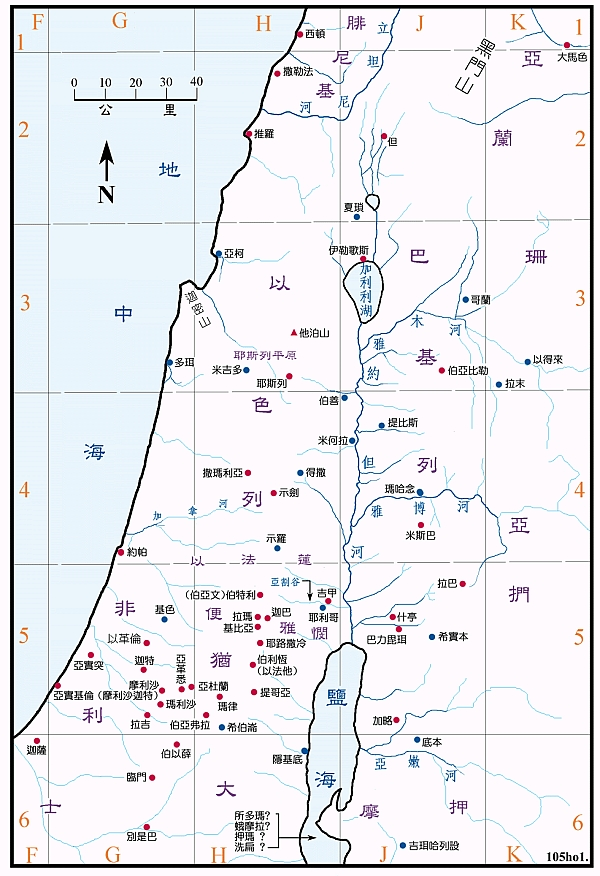
\includegraphics[width=6.in]{DXianZhiFigs/MiJiaFig/MiJia}
%\caption{彌迦書地名}
%\label{fig:sub1}
\end{figure}



\section{以色列與猶大拜偶像 1-2}

\subsection{先知得神的默示,主要审判以色列與猶大拜偶像的罪 1:1-7}
當猶大王約坦、亞哈斯、希西家在位的時候，摩利沙人彌迦得耶和華的默示，論撒馬利亞和耶路撒冷。

%\subsection{主要审判雅各家的罪過 1:2-5}
萬民哪，你們都要聽！地和其上所有的，也都要側耳而聽！主耶和華從他的聖殿要見證你們的不是。 3 看哪，耶和華出了他的居所，降臨步行地的高處。 4 眾山在他以下必消化，諸谷必崩裂，如蠟化在火中，如水沖下山坡。 5 這都因雅各的罪過，以色列家的罪惡。

%\subsection{主要审判拜偶像的罪 1:6-7}
雅各的罪過在哪裡呢？豈不是在撒馬利亞嗎？猶大的丘壇在哪裡呢？豈不是在耶路撒冷嗎？ 6 「所以，我必使撒馬利亞變為田野的亂堆，又作為種葡萄之處；也必將她的石頭倒在谷中，露出根基來。 7 她一切雕刻的偶像必被打碎，她所得的財物必被火燒，所有的偶像我必毀滅，因為是從妓女雇價所聚來的，後必歸為妓女的雇價。」


\subsection{先知為此號啕,多方居民為此哀哭 1:8-16}
先知說：因此我必大聲哀號，赤腳露體而行；又要呼號如野狗，哀鳴如鴕鳥。 9 因為撒馬利亞的傷痕無法醫治，延及猶大和耶路撒冷我民的城門。 10 不要在迦特報告這事，總不要哭泣；我在伯亞弗拉滾於灰塵之中。 11 「\textcolor{red}{沙斐}的居民哪，你們要赤身蒙羞過去。\textcolor{red}{撒南}的居民不敢出來，\textcolor{red}{伯以薛}人的哀哭使你們無處可站。 12 \textcolor{red}{瑪律}的居民心甚憂急，切望得好處，因為災禍從耶和華那裡臨到耶路撒冷的城門。 13 \textcolor{red}{拉吉}的居民哪，要用快馬套車，錫安民(女子)的罪由你而起，以色列人的罪過在你那裡顯出。 14 \textcolor{red}{猶大}啊，你要將禮物送給摩利設迦特。\textcolor{red}{亞革悉}的眾族必用詭詐待以色列諸王。 15 \textcolor{red}{瑪利沙}的居民哪，我必使那奪取你的來到你這裡。\textcolor{red}{以色列}的尊貴人(榮耀)必到亞杜蘭。 16 \textcolor{red}{猶大}啊，要為你所喜愛的兒女剪除你的頭髮，使頭光禿。要大大地光禿，如同禿鷹，因為他們都被擄去離開你。」

\section{以色列與猶大其他的罪 2}

\subsection{惡人欺壓抢奪,必受災禍 2:1-6}
%\subsubsection{惡人肆行欺虐 2:1-3}
禍哉，那些在床上圖謀罪孽、造做奸惡的！天一發亮，因手有能力就行出來了。 2 他們貪圖田地就占據，貪圖房屋便奪取。他們欺壓人，霸占房屋和產業。 

%\subsubsection{惡人必受災禍 2:4-6}
3 所以耶和華如此說：「我籌劃災禍降於這族，這禍在你們的頸項上不能解脫，你們也不能昂首而行，因為這時勢是惡的。

「到那日，必有人向你們提起悲慘的哀歌，譏刺說：『我們全然敗落了！耶和華將我們的份轉歸別人。何竟使這份離開我們？他將我們的田地分給悖逆的人。』 5 所以在耶和華的會中，你必沒有人拈鬮拉準繩。

\subsection{禁止先知說預言，立假先知的禍，雅各蒙恩旋返如羊歸牢 2:6-13}
%\subsubsection{恶待先知說預言 2:4-6}
他們（假先知）說：『你們不可說預言！不可向這些人說預言，不住地羞辱我們。』 

7 雅各家啊，豈可說耶和華的心不忍耐（心腸狹窄）嗎？這些事是他所行的嗎？我耶和華的言語，豈不是與行動正直的人有益嗎？ 8 然而近來我的民興起如仇敵，從那些安然經過不願打仗之人身上剝去外衣。 9 你們將我民中的婦人從安樂家中趕出，又將我的榮耀從她們的小孩子盡行奪去。 10 你們起來去吧！這不是你們安息之所。因為汙穢使人（地）毀滅，而且大大毀滅。 

11 若有人心存虛假，用謊言說『我要向你們預言得清酒和濃酒』，那人就必做這民的先知！

%\subsubsection{雅各蒙恩旋返如羊歸牢 2:12-16}

「雅各家啊，我必要聚集你們，必要招聚以色列剩下的人，安置在一處，如波斯拉的羊，又如草場上的羊群。因為人數眾多，就必大大喧嘩。 13 開路的（破城的）在他們前面上去，他們直闖過城門，從城門出去。他們的王在前面行，耶和華引導他們。」



\section{劝勉 3}
\subsection{劝勉雅各首領和官長 3:1-4}
我說：雅各的首領，以色列家的官長啊，你們要聽！你們不當知道公平嗎？ 2 你們惡善好惡，從人身上剝皮，從人骨頭上剔肉。 3 吃我民的肉，剝他們的皮，打折他們的骨頭，分成塊子像要下鍋，又像釜中的肉。 4 到了遭災的時候，這些人必哀求耶和華，他卻不應允他們。那時他必照他們所行的惡事，向他們掩面。

\subsection{真假先知 3:5-8}
論到使我民走差路的先知，他們牙齒有所嚼的，他們就呼喊說「平安了！」，凡不供給他們吃的，他們就預備攻擊他（說必遭遇刀兵）。耶和華如此說： 6 「你們必遭遇黑夜，以致不見異象；又必遭遇幽暗，以致不能占卜。日頭必向你們沉落，白晝變為黑暗。 7 先見必抱愧，占卜的必蒙羞，都必摀著嘴唇，因為神不應允他們。」 

8 至於我，我藉耶和華的靈，滿有力量、公平、才能，可以向雅各說明他的過犯，向以色列指出他的罪惡

\subsection{劝勉首領，官長，祭司，先知 3:9-12}
雅各家的首領，以色列家的官長啊，當聽我的話！你們厭惡公平，在一切事上屈枉正直， 10 以人血建立錫安，以罪孽建造耶路撒冷。 11 首領為賄賂行審判，祭司為雇價施訓誨，先知為銀錢行占卜，他們卻倚賴耶和華說：「耶和華不是在我們中間嗎？災禍必不臨到我們。」 12 所以因你們的緣故，錫安必被耕種像一塊田，耶路撒冷必變為亂堆，這殿的山必像叢林的高處。



\section{末后的预言 4}
\subsection{末日的平安 4:1-8}
\subsubsection{末日萬民必歸錫安，萬國不相攻，耶和華做王錫安到永遠 4:1-8}
末後的日子，耶和華殿的山必堅立超乎諸山，高舉過於萬嶺，萬民都要流歸這山。 2 必有許多國的民前往，說：「來吧！我們登耶和華的山，奔雅各神的殿。主必將他的道教訓我們，我們也要行他的路，因為訓誨必出於錫安，耶和華的言語必出於耶路撒冷。」


%\subsubsection{主使萬民綏安國不相攻 4:3-5}
他必在多國的民中施行審判，為遠方強盛的國斷定是非。他們要將刀打成犁頭，把槍打成鐮刀。這國不舉刀攻擊那國，他們也不再學習戰事。 4 人人都要坐在自己葡萄樹下和無花果樹下，無人驚嚇。這是萬軍之耶和華親口說的。 5 萬民各奉己神的名而行，我們卻永永遠遠奉耶和華我們神的名而行。


%\subsubsection{耶和華做王錫安國祚永遠 4:6-8}
耶和華說：「到那日，我必聚集瘸腿的，招聚被趕出的和我所懲治的。 7 我必使瘸腿的為餘剩之民，使趕到遠方的為強盛之民。耶和華要在錫安山做王治理他們，從今直到永遠。 8 你這羊群的高臺，錫安城(女子)的山哪，從前的權柄，就是耶路撒冷民 (女子)的國權，必歸於你。


\subsection{錫安被諸國集攻却要得勝 4:9-13}
%\subsubsection{錫安被諸國集攻 4:9-12}
 「現在你為何大聲哭號呢？疼痛抓住你，彷彿產難的婦人，是因你中間沒有君王嗎？你的謀士滅亡了嗎？ 10 錫安的民(女子)哪，你要疼痛劬勞，彷彿產難的婦人。因為你必從城裡出來，住在田野，到巴比倫去。在那裡要蒙解救，在那裡耶和華必救贖你脫離仇敵的手。 11 現在有許多國的民聚集攻擊你，說：『願錫安被玷汙，願我們親眼見她遭報！』 12 他們卻不知道耶和華的意念，也不明白他的籌劃：他聚集他們，好像把禾捆聚到禾場一樣。

%\subsubsection{錫安得勝 4:13}
「錫安的民(女子)哪，起來踹穀吧！我必使你的角成為鐵，使你的蹄成為銅。你必打碎多國的民，將他們的財獻於耶和華，將他們的貨獻於普天下的主。」

\subsubsection{掌權的由伯利恆而出搭救餘民,除滅偶像施報不聽從的列國 5:1-15}
\begin{table}[H]
\centering
\begin{tabular}{p{3.75cm}|p{5cm}|p{3.75cm}|p{4.150cm}}\hline\hline
\multicolumn{1}{c|}{掌權的由伯利恆而出}&\multicolumn{1}{c|}{牧養拯救境内羊群4-6}&\multicolumn{1}{c|}{搭救餘民7-9}&\multicolumn{1}{c}{除滅偶像施報列國10-15}\\\hline
成群的民(女子)哪，現在你要聚集成隊！因為仇敵圍攻我們，要用杖擊打以色列審判者的臉。「伯利恆以法他啊，你在猶大諸城中為小，將來必有一位從你那裡出來，在以色列中為我做掌權的。他的根源從亙古，從太初就有。」耶和華必將以色列人交付敵人，直等那生產的婦人生下子來。
&\multirow{1}{5.25cm}{那時，掌權者(他)其餘的弟兄必歸到以色列人那裡
他必起來，倚靠耶和華的大能並耶和華他神之名的威嚴，牧養他的羊群。他們要安然居住，因為他必日見尊大，直到地極。這位必做我們的平安。當亞述人進入我們的地境，踐踏宮殿的時候，我們就立起七個牧者、八個首領攻擊他。他們必用刀劍毀壞亞述地和寧錄地的關口。亞述人進入我們的地境踐踏的時候，他必拯救我們。}
&\multirow{1}{4.cm}{雅各餘剩的人必在多國的民中，如從耶和華那裡降下的露水，又如甘霖降在草上；不仗賴人力，也不等候世人之功。雅各餘剩的人必在多國多民中，如林間百獸中的獅子，又如少壯獅子在羊群中。他若經過，就必踐踏撕裂，無人搭救。願你的手舉起高過敵人，願你的仇敵都被剪除！}
&耶和華說：「到那日,我必從你中間剪除馬匹,毀壞車輛。也必從你國中除滅城邑,拆毀一切的保障。又必除掉你手中的邪術,你那裡也不再有占卜的。我必從你中間除滅雕刻的偶像和柱像,你就不再跪拜自己手所造的。我必從你中間拔出木偶,又毀滅你的城邑。我也必在怒氣和憤怒中,向那不聽從的列國施報。」\\\hline
\end{tabular}
\end{table}



\section{責民負恩,愚頑以為獻祭可蒙主悅,言行不義,從亞哈家惡規 6}

%\subsection{責民負恩 6:1-5}
以色列人哪，當聽耶和華的話：「要起來，向山嶺爭辯，使岡陵聽你的話！ 2 山嶺和地永久的根基啊，要聽耶和華爭辯的話，因為耶和華要與他的百姓爭辯，與以色列爭論。 3 我的百姓啊，我向你做了什麼呢？我在什麼事上使你厭煩？你可以對我證明。 4 我曾將你從埃及地領出來，從做奴僕之家救贖你，我也差遣摩西、亞倫和米利暗在你前面行。 5 我的百姓啊，你們當追念摩押王巴勒所設的謀和比珥的兒子巴蘭回答他的話，並你們從什亭到吉甲所遇見的事，好使你們知道耶和華公義的作為。」

%\subsection{責民愚頑以為獻祭可蒙主悅 6:6-8}
我朝見耶和華，在至高神面前跪拜，當獻上什麼呢？豈可獻一歲的牛犢為燔祭嗎？ 7 耶和華豈喜悅千千的公羊，或是萬萬的油河嗎？我豈可為自己的罪過獻我的長子嗎？為心中的罪惡獻我身所生的嗎？ 8 世人哪！耶和華已指示你何為善。他向你所要的是什麼呢？只要你行公義，好憐憫，存謙卑的心，與你的神同行

%\subsection{責民言行不義 6:9-13}
耶和華向這城呼叫，智慧人必敬畏他的名。「你們當聽是誰派定刑杖的懲罰。 10 惡人家中不仍有非義之財和可惡的小升斗嗎？ 11 我若用不公道的天平和囊中詭詐的法碼，豈可算為清潔呢？ 12 城裡的富戶滿行強暴，其中的居民也說謊言，口中的舌頭是詭詐的。 13 因此我擊打你，使你的傷痕甚重，使你因你的罪惡荒涼。


%\subsection{責民從亞哈家惡規 6:14-16}

你要吃卻吃不飽，你的虛弱必顯在你中間。你必挪去卻不得救護，所救護的我必交給刀劍。 15 你必撒種卻不得收割，踹橄欖卻不得油抹身，踹葡萄卻不得酒喝。 16 因為你守暗利的惡規，行亞哈家一切所行的，順從他們的計謀。因此，我必使你荒涼，使你的居民令人嗤笑，你們也必擔當我民的羞辱。」

\section{祷告-嘆義人死亡,人心唯惡是趨,勿恃世人唯賴等候神,求主復施恩惠止怒赦罪 7}

%\subsection{哀嘆義人死亡 7:1-5}
哀哉！我（或指以色列）好像夏天的果子已被收盡，又像摘了葡萄所剩下的，沒有一掛可吃的，我心羨慕初熟的無花果。 2 地上虔誠人滅盡，世間沒有正直人。各人埋伏要殺人流血，都用網羅獵取弟兄。

%\subsection{人心唯惡是趨 7:1-5}
他們雙手作惡，君王徇情面，審判官要賄賂，位分大的吐出惡意，都彼此結聯行惡。 4 他們最好的不過是蒺藜，最正直的不過是荊棘籬笆。你守望者說降罰的日子已經來到，他們必擾亂不安

%\subsection{勿恃世人唯賴神 7:1-5}
不要倚賴鄰舍，不要信靠密友，要守住你的口，不要向你懷中的妻提說。 6 因為兒子藐視父親，女兒抗拒母親，媳婦抗拒婆婆，人的仇敵就是自己家裡的人。


%\subsection{先知祷告要等候神 7:6-13}
至於我，我要仰望耶和華，要等候那救我的神，我的神必應允我。 8 我的仇敵啊，不要向我誇耀！我雖跌倒，卻要起來；我雖坐在黑暗裡，耶和華卻做我的光。 9 我要忍受耶和華的惱怒，因我得罪了他。直等他為我辨屈，為我申冤，他必領我到光明中，我必得見他的公義。 10 那時，我的仇敵，就是曾對我說「耶和華你神在哪裡」的，他一看見這事就被羞愧遮蓋。我必親眼見他遭報，他必被踐踏，如同街上的泥土。 11 以色列啊，日子必到，你的牆垣必重修。到那日，你的境界必開展（命令必傳到遠方）。 12 當那日，人必從亞述，從埃及的城邑，從埃及到大河，從這海到那海，從這山到那山，都歸到你這裡。 13 然而，這地因居民的緣故，又因他們行事的結果，必然荒涼


%\subsection{求主復施恩惠 7:14-17}

求耶和華在迦密山的樹林中，用你的杖牧放你獨居的民，就是你產業的羊群。求你容他們在巴珊和基列得食物，像古時一樣。 15 耶和華說：「我要把奇事顯給他們看，好像出埃及地的時候一樣。」 16 列國看見這事，就必為自己的勢力慚愧。他們必用手摀口，掩耳不聽。 17 他們必舔土如蛇，又如土中腹行的物，戰戰兢兢地出他們的營寨。他們必戰懼投降耶和華，也必因我們的神而懼怕。

%\subsection{求主止怒赦罪 7:18-20}

神啊，有何神像你？赦免罪孽，饒恕你產業之餘民的罪過。不永遠懷怒，喜愛施恩。 19 必再憐憫我們，將我們的罪孽踏在腳下，又將我們的一切罪投於深海。 20 你必按古時起誓應許我們列祖的話，向雅各發誠實，向亞伯拉罕施慈愛。











